\section{Validation (Preliminary results)}
\label{sec:validation}
Here we follow some cases from the 2nd High-Order Workshop.

\subsection{Flat Plate}

\subsection{Circular Cylinder}
From David's thesis.



%\subsubsection{Vortex transport by uniform flow (2D)}
%\subsubsection{Transonic Ringleb Flow (2D)}
%\subsubsection{Flow over an Analytical Body of Revolution (3D)}

\subsection{RANS NACA 0012}

\subsection{SD7003 airfoil at 4$\degr$ angle of attack}
From David's thesis\cite{williams2013thesis}
\subsection{SD7003 wing section at 4$\degr$ angle of attack}
From David's thesis.
%\subsubsection{Laminar Flow around a Delta Wing}

\subsection{DNS of the Taylor-Green Vortex at Re = 1,600}

\begin{figure}
\centering
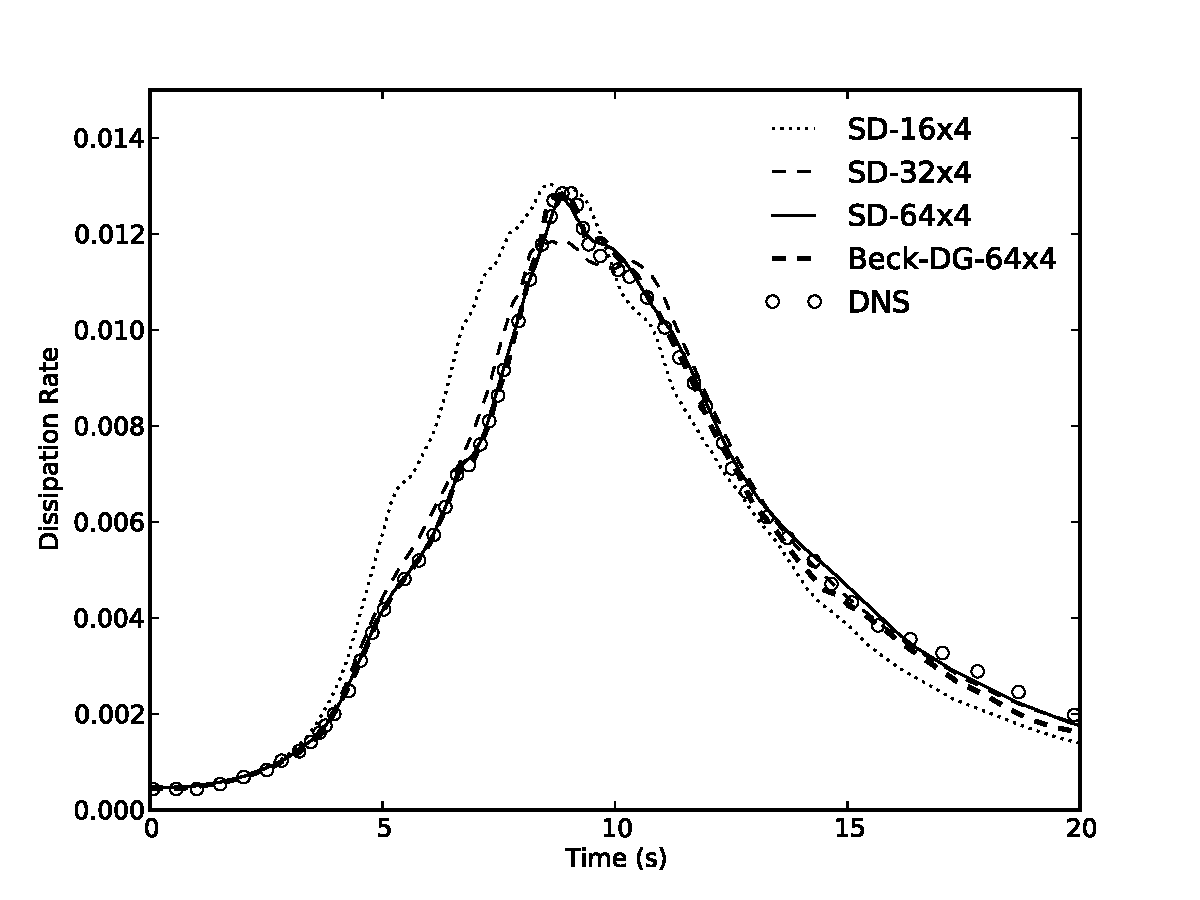
\includegraphics[height=60mm]{./figures/dissrate-hex-mesh-small.pdf} \\
\caption{LES of Tyalor-Green Vortex at Re=1,600\cite{bull2013a}}
\label{fig:setup}
\end{figure}


\subsection{DNS of Decaying Homogeneous Turbulence}
To be done by Manuel
\subsection{LES of Decaying Homogeneous Turbulence}
To be done by Manuel

